% Options for packages loaded elsewhere
\PassOptionsToPackage{unicode}{hyperref}
\PassOptionsToPackage{hyphens}{url}
%
\documentclass[
]{article}
\usepackage{amsmath,amssymb}
\usepackage{iftex}
\ifPDFTeX
  \usepackage[T1]{fontenc}
  \usepackage[utf8]{inputenc}
  \usepackage{textcomp} % provide euro and other symbols
\else % if luatex or xetex
  \usepackage{unicode-math} % this also loads fontspec
  \defaultfontfeatures{Scale=MatchLowercase}
  \defaultfontfeatures[\rmfamily]{Ligatures=TeX,Scale=1}
\fi
\usepackage{lmodern}
\ifPDFTeX\else
  % xetex/luatex font selection
\fi
% Use upquote if available, for straight quotes in verbatim environments
\IfFileExists{upquote.sty}{\usepackage{upquote}}{}
\IfFileExists{microtype.sty}{% use microtype if available
  \usepackage[]{microtype}
  \UseMicrotypeSet[protrusion]{basicmath} % disable protrusion for tt fonts
}{}
\makeatletter
\@ifundefined{KOMAClassName}{% if non-KOMA class
  \IfFileExists{parskip.sty}{%
    \usepackage{parskip}
  }{% else
    \setlength{\parindent}{0pt}
    \setlength{\parskip}{6pt plus 2pt minus 1pt}}
}{% if KOMA class
  \KOMAoptions{parskip=half}}
\makeatother
\usepackage{xcolor}
\usepackage[margin=1in]{geometry}
\usepackage{color}
\usepackage{fancyvrb}
\newcommand{\VerbBar}{|}
\newcommand{\VERB}{\Verb[commandchars=\\\{\}]}
\DefineVerbatimEnvironment{Highlighting}{Verbatim}{commandchars=\\\{\}}
% Add ',fontsize=\small' for more characters per line
\usepackage{framed}
\definecolor{shadecolor}{RGB}{248,248,248}
\newenvironment{Shaded}{\begin{snugshade}}{\end{snugshade}}
\newcommand{\AlertTok}[1]{\textcolor[rgb]{0.94,0.16,0.16}{#1}}
\newcommand{\AnnotationTok}[1]{\textcolor[rgb]{0.56,0.35,0.01}{\textbf{\textit{#1}}}}
\newcommand{\AttributeTok}[1]{\textcolor[rgb]{0.13,0.29,0.53}{#1}}
\newcommand{\BaseNTok}[1]{\textcolor[rgb]{0.00,0.00,0.81}{#1}}
\newcommand{\BuiltInTok}[1]{#1}
\newcommand{\CharTok}[1]{\textcolor[rgb]{0.31,0.60,0.02}{#1}}
\newcommand{\CommentTok}[1]{\textcolor[rgb]{0.56,0.35,0.01}{\textit{#1}}}
\newcommand{\CommentVarTok}[1]{\textcolor[rgb]{0.56,0.35,0.01}{\textbf{\textit{#1}}}}
\newcommand{\ConstantTok}[1]{\textcolor[rgb]{0.56,0.35,0.01}{#1}}
\newcommand{\ControlFlowTok}[1]{\textcolor[rgb]{0.13,0.29,0.53}{\textbf{#1}}}
\newcommand{\DataTypeTok}[1]{\textcolor[rgb]{0.13,0.29,0.53}{#1}}
\newcommand{\DecValTok}[1]{\textcolor[rgb]{0.00,0.00,0.81}{#1}}
\newcommand{\DocumentationTok}[1]{\textcolor[rgb]{0.56,0.35,0.01}{\textbf{\textit{#1}}}}
\newcommand{\ErrorTok}[1]{\textcolor[rgb]{0.64,0.00,0.00}{\textbf{#1}}}
\newcommand{\ExtensionTok}[1]{#1}
\newcommand{\FloatTok}[1]{\textcolor[rgb]{0.00,0.00,0.81}{#1}}
\newcommand{\FunctionTok}[1]{\textcolor[rgb]{0.13,0.29,0.53}{\textbf{#1}}}
\newcommand{\ImportTok}[1]{#1}
\newcommand{\InformationTok}[1]{\textcolor[rgb]{0.56,0.35,0.01}{\textbf{\textit{#1}}}}
\newcommand{\KeywordTok}[1]{\textcolor[rgb]{0.13,0.29,0.53}{\textbf{#1}}}
\newcommand{\NormalTok}[1]{#1}
\newcommand{\OperatorTok}[1]{\textcolor[rgb]{0.81,0.36,0.00}{\textbf{#1}}}
\newcommand{\OtherTok}[1]{\textcolor[rgb]{0.56,0.35,0.01}{#1}}
\newcommand{\PreprocessorTok}[1]{\textcolor[rgb]{0.56,0.35,0.01}{\textit{#1}}}
\newcommand{\RegionMarkerTok}[1]{#1}
\newcommand{\SpecialCharTok}[1]{\textcolor[rgb]{0.81,0.36,0.00}{\textbf{#1}}}
\newcommand{\SpecialStringTok}[1]{\textcolor[rgb]{0.31,0.60,0.02}{#1}}
\newcommand{\StringTok}[1]{\textcolor[rgb]{0.31,0.60,0.02}{#1}}
\newcommand{\VariableTok}[1]{\textcolor[rgb]{0.00,0.00,0.00}{#1}}
\newcommand{\VerbatimStringTok}[1]{\textcolor[rgb]{0.31,0.60,0.02}{#1}}
\newcommand{\WarningTok}[1]{\textcolor[rgb]{0.56,0.35,0.01}{\textbf{\textit{#1}}}}
\usepackage{graphicx}
\makeatletter
\def\maxwidth{\ifdim\Gin@nat@width>\linewidth\linewidth\else\Gin@nat@width\fi}
\def\maxheight{\ifdim\Gin@nat@height>\textheight\textheight\else\Gin@nat@height\fi}
\makeatother
% Scale images if necessary, so that they will not overflow the page
% margins by default, and it is still possible to overwrite the defaults
% using explicit options in \includegraphics[width, height, ...]{}
\setkeys{Gin}{width=\maxwidth,height=\maxheight,keepaspectratio}
% Set default figure placement to htbp
\makeatletter
\def\fps@figure{htbp}
\makeatother
\setlength{\emergencystretch}{3em} % prevent overfull lines
\providecommand{\tightlist}{%
  \setlength{\itemsep}{0pt}\setlength{\parskip}{0pt}}
\setcounter{secnumdepth}{-\maxdimen} % remove section numbering
\ifLuaTeX
  \usepackage{selnolig}  % disable illegal ligatures
\fi
\IfFileExists{bookmark.sty}{\usepackage{bookmark}}{\usepackage{hyperref}}
\IfFileExists{xurl.sty}{\usepackage{xurl}}{} % add URL line breaks if available
\urlstyle{same}
\hypersetup{
  pdftitle={tumor classification with machine learning methods},
  pdfauthor={Gordon Ma},
  hidelinks,
  pdfcreator={LaTeX via pandoc}}

\title{tumor classification with machine learning methods}
\author{Gordon Ma}
\date{}

\begin{document}
\maketitle

\hypertarget{introduction}{%
\section{Introduction}\label{introduction}}

\hypertarget{what-is-gene-expression}{%
\subsection{What is gene expression?}\label{what-is-gene-expression}}

Gene expression is the process by which information from a gene is used
to synthesize functional gene products, such as proteins or RNA
molecules. It involves the transcription of the gene's DNA into RNA and
the translation of that RNA into a protein. The expression of a gene is
the amount of its mRNA molecule that has been detected in a gene. The
higher the expression indicates the higher abundance of mRNA detected.

In this project, we analyze the data set that comes from a paper by
\href{http://www.ncbi.nlm.nih.gov/geo/query/acc.cgi?acc=GSE23177}{Smeets
et al.~2010}, who studied Affymetrix expression profiles from primary
breast tumours. The authors were interested in whether tumors which had
spread to lymph nodes (LN positive, generally a bad sign) have different
gene expression profiles than LN negative tumors. If so, how can a gene
expression signature be used to predict tumor class?

Their data set contains 24236 genes on 116 samples. The status of the
lymph node is known for each sample, with 59 LN positive and 57 LN
negative. Samples were divided into two parts: 96 samples (48 LN
positive and 48 LN negative) were used as a ``training'' set and 20
samples (11 LN positive and 9 LN negative) were used as a ``test'' set.
There is also a quantitative measure, ``LnRatio'', the fraction of
affected lymph nodes, presumably reflecting ``how bad'' the LnStatus is.

\hypertarget{data-preparation}{%
\subsection{Data Preparation}\label{data-preparation}}

Install the following packages from Bioconductor: \texttt{CMA} and
\texttt{GEOquery}. \texttt{CMA} is the package for classification
methods using gene expression data, and \texttt{GEOquery} is the used to
query biological data from the \href{https://www.ncbi.nlm.nih.gov/}{NCBI
website}. We also install the following packages from CRAN:
\texttt{ROCR}, \texttt{car}, \texttt{e1071} (for SVM), and
\texttt{glmnet(Generalized\ linear\ model)} along with their
dependencies.

\begin{Shaded}
\begin{Highlighting}[]
\FunctionTok{library}\NormalTok{(tidyverse)}\CommentTok{\#Data wrangling and visualization}
\FunctionTok{library}\NormalTok{(limma) }
\FunctionTok{library}\NormalTok{(ROCR)}
\FunctionTok{library}\NormalTok{(CMA)}
\FunctionTok{library}\NormalTok{(class) }
\FunctionTok{library}\NormalTok{(pROC)}
\end{Highlighting}
\end{Shaded}

\begin{verbatim}
## Warning: package 'pROC' was built under R version 4.3.3
\end{verbatim}

\begin{Shaded}
\begin{Highlighting}[]
\FunctionTok{library}\NormalTok{(GEOquery) }\CommentTok{\#Query the data }
\end{Highlighting}
\end{Shaded}

First, let's retrieve our data set from GEO with \texttt{getGEO} from
\texttt{GEOquery} package. The detail of the study is published on the
\href{comes\%20from\%20a\%20paper\%20by\%20Smeets\%20et\%20al.\%202010}{website}.

\begin{Shaded}
\begin{Highlighting}[]
\CommentTok{\# Returns a list of expressionsets}
\NormalTok{datgeo }\OtherTok{\textless{}{-}} \FunctionTok{getGEO}\NormalTok{(}\StringTok{\textquotesingle{}GSE23177\textquotesingle{}}\NormalTok{, }\AttributeTok{GSEMatrix =} \ConstantTok{TRUE}\NormalTok{, }\AttributeTok{AnnotGPL =} \ConstantTok{TRUE}\NormalTok{) }
\NormalTok{dat }\OtherTok{\textless{}{-}}\NormalTok{ datgeo[[}\DecValTok{1}\NormalTok{]]   }\CommentTok{\#Note that dat is an ExpressionSet}
\end{Highlighting}
\end{Shaded}

\begin{Shaded}
\begin{Highlighting}[]
\NormalTok{dat}
\end{Highlighting}
\end{Shaded}

\begin{verbatim}
## ExpressionSet (storageMode: lockedEnvironment)
## assayData: 24236 features, 116 samples 
##   element names: exprs 
## protocolData: none
## phenoData
##   sampleNames: GSM570498 GSM570499 ... GSM570613 (116 total)
##   varLabels: title geo_accession ... patient type:ch1 (49 total)
##   varMetadata: labelDescription
## featureData
##   featureNames: 1007_s_at 1053_at ... 91952_at (24236 total)
##   fvarLabels: ID Gene title ... GO:Component ID (21 total)
##   fvarMetadata: Column Description labelDescription
## experimentData: use 'experimentData(object)'
##   pubMedIds: 21116709 
## Annotation: GPL570
\end{verbatim}

The expression matrix contains the sample IDs and their corresponding
gene expression profiles, which we can access from
the~\texttt{ExpressionSet}~object with~\texttt{exprs()}. Essentially,
each column is a different sample(a tissue, under treatment,
environment, etc) and each row is a gene(or a probe).

\begin{Shaded}
\begin{Highlighting}[]
\CommentTok{\#Print out the small subset of the expression matrix}
\FunctionTok{exprs}\NormalTok{(dat)[}\DecValTok{1}\SpecialCharTok{:}\DecValTok{10}\NormalTok{, }\DecValTok{1}\SpecialCharTok{:}\DecValTok{5}\NormalTok{]}
\end{Highlighting}
\end{Shaded}

\begin{verbatim}
##              GSM570498 GSM570499 GSM570500 GSM570501 GSM570502
## 1007_s_at     9.972979 10.905187 10.277672  9.675721 10.136213
## 1053_at       7.817832  7.079229  6.930580  7.250610  7.701002
## 117_at        8.725469  6.036008  5.481603  6.704801  6.704787
## 121_at        7.368854  6.575936  6.917470  6.533265  6.443367
## 1294_at       6.554170  6.764196  6.891401  6.609946  7.276797
## 1316_at       3.943299  4.889293  3.614283  4.496297  4.499382
## 1405_i_at     6.607460  6.640302  6.794514  6.507395  6.969491
## 1431_at       4.274017  3.932747  2.324288  2.355886  3.722960
## 1438_at       5.961952  5.699793  7.506902  6.775789  6.198671
## 1552256_a_at  8.228385  8.268530  8.039264  7.977523  8.480362
\end{verbatim}

The properties associated with each sample are stored in the sample
metadata, which can be accessed using the \texttt{pData()} function. For
instance, the following code returns whether each sample is LN positive
or LN negative, test or training group.

\begin{Shaded}
\begin{Highlighting}[]
\CommentTok{\# extract only those variables of interest }
\FunctionTok{pData}\NormalTok{(dat) }\OtherTok{\textless{}{-}} \FunctionTok{pData}\NormalTok{(dat) }\SpecialCharTok{\%\textgreater{}\%}
  \FunctionTok{rename}\NormalTok{(}\AttributeTok{sample\_id =}\NormalTok{ geo\_accession,}
         \AttributeTok{LnStatus =}\NormalTok{ characteristics\_ch1}\FloatTok{.2}\NormalTok{, }\CommentTok{\#disease status}
         \AttributeTok{LnRatio =}\NormalTok{ characteristics\_ch1}\FloatTok{.3}\NormalTok{, }\CommentTok{\#the proportion of the infected node}
         \AttributeTok{Set =}\NormalTok{ characteristics\_ch1) }\SpecialCharTok{\%\textgreater{}\%} \CommentTok{\#Which are training and testing set }
  \FunctionTok{mutate}\NormalTok{(}\AttributeTok{LnStatus =} \FunctionTok{factor}\NormalTok{(}\FunctionTok{gsub}\NormalTok{(}\StringTok{"ln: "}\NormalTok{, }\StringTok{""}\NormalTok{, LnStatus))) }\SpecialCharTok{\%\textgreater{}\%}
  \FunctionTok{mutate}\NormalTok{(}\AttributeTok{LnRatio =} \FunctionTok{as.numeric}\NormalTok{(}\FunctionTok{gsub}\NormalTok{(}\StringTok{"lnratio: "}\NormalTok{, }\StringTok{""}\NormalTok{, LnRatio))) }\SpecialCharTok{\%\textgreater{}\%}
  \FunctionTok{mutate}\NormalTok{(}\AttributeTok{Set =} \FunctionTok{ifelse}\NormalTok{(Set }\SpecialCharTok{==} \StringTok{"patient type: training set"}\NormalTok{, }\StringTok{"training"}\NormalTok{, }\StringTok{"test"}\NormalTok{))}

\FunctionTok{str}\NormalTok{(}\FunctionTok{pData}\NormalTok{(dat) }\SpecialCharTok{\%\textgreater{}\%} \FunctionTok{select}\NormalTok{(sample\_id, LnStatus, LnRatio, Set) )}
\end{Highlighting}
\end{Shaded}

\begin{verbatim}
## 'data.frame':    116 obs. of  4 variables:
##  $ sample_id: chr  "GSM570498" "GSM570499" "GSM570500" "GSM570501" ...
##  $ LnStatus : Factor w/ 2 levels "neg","pos": 1 1 1 1 1 1 1 1 1 2 ...
##  $ LnRatio  : num  0 0 0 0 0 0 0 0 0 0.5 ...
##  $ Set      : chr  "test" "test" "test" "test" ...
\end{verbatim}

Next, let's split the \texttt{ExpressionSet} object into two different
parts - one for the training and one for the test set.

\begin{Shaded}
\begin{Highlighting}[]
\CommentTok{\# split the ExpressionSet into training and test sets. }
\FunctionTok{table}\NormalTok{(}\FunctionTok{pData}\NormalTok{(dat)}\SpecialCharTok{$}\NormalTok{Set)}
\end{Highlighting}
\end{Shaded}

\begin{verbatim}
## 
##     test training 
##       20       96
\end{verbatim}

\begin{Shaded}
\begin{Highlighting}[]
\NormalTok{train.es }\OtherTok{\textless{}{-}}\NormalTok{ dat[, dat}\SpecialCharTok{$}\NormalTok{Set }\SpecialCharTok{==} \StringTok{"training"}\NormalTok{]}
\NormalTok{test.es }\OtherTok{\textless{}{-}}\NormalTok{ dat[ , dat}\SpecialCharTok{$}\NormalTok{Set }\SpecialCharTok{==} \StringTok{"test"}\NormalTok{]}
\end{Highlighting}
\end{Shaded}

\begin{Shaded}
\begin{Highlighting}[]
\CommentTok{\#Look at the number of case/control}
\FunctionTok{table}\NormalTok{(train.es}\SpecialCharTok{$}\NormalTok{LnStatus)}
\end{Highlighting}
\end{Shaded}

\begin{verbatim}
## 
## neg pos 
##  48  48
\end{verbatim}

\begin{Shaded}
\begin{Highlighting}[]
\FunctionTok{table}\NormalTok{(test.es}\SpecialCharTok{$}\NormalTok{LnStatus)}
\end{Highlighting}
\end{Shaded}

\begin{verbatim}
## 
## neg pos 
##   9  11
\end{verbatim}

Now, we can do some exploratory analysis of the data before trying some
classification methods.

\begin{Shaded}
\begin{Highlighting}[]
\CommentTok{\# look at the expression of 3 randomly picked genes in both training and test sets}
\FunctionTok{set.seed}\NormalTok{(}\DecValTok{1234}\NormalTok{)}
\NormalTok{rangenes }\OtherTok{\textless{}{-}} \FunctionTok{sample}\NormalTok{(}\DecValTok{1}\SpecialCharTok{:}\FunctionTok{nrow}\NormalTok{(dat), }\AttributeTok{size =} \DecValTok{3}\NormalTok{) }

\CommentTok{\# function to create tidy data table of expression and metadata}
\NormalTok{toLonger }\OtherTok{\textless{}{-}} \ControlFlowTok{function}\NormalTok{(expset) \{}
    \FunctionTok{stopifnot}\NormalTok{(}\FunctionTok{class}\NormalTok{(expset) }\SpecialCharTok{==} \StringTok{"ExpressionSet"}\NormalTok{)}
    
\NormalTok{    expressionMatrix }\OtherTok{\textless{}{-}}\NormalTok{ longExpressionMatrix }\OtherTok{\textless{}{-}} \FunctionTok{exprs}\NormalTok{(expset) }\SpecialCharTok{\%\textgreater{}\%} 
      \FunctionTok{as.data.frame}\NormalTok{() }\SpecialCharTok{\%\textgreater{}\%}
      \FunctionTok{rownames\_to\_column}\NormalTok{(}\StringTok{"gene"}\NormalTok{) }\SpecialCharTok{\%\textgreater{}\%}
      \FunctionTok{pivot\_longer}\NormalTok{(}\AttributeTok{cols =} \SpecialCharTok{!}\NormalTok{gene, }
                   \AttributeTok{values\_to =} \StringTok{"expression"}\NormalTok{,}
                   \AttributeTok{names\_to =} \StringTok{"sample\_id"}\NormalTok{) }\SpecialCharTok{\%\textgreater{}\%}
      \FunctionTok{left\_join}\NormalTok{(}\FunctionTok{pData}\NormalTok{(expset), }\AttributeTok{by =} \StringTok{"sample\_id"}\NormalTok{)}
  \FunctionTok{return}\NormalTok{(expressionMatrix)}
\NormalTok{\}}

\FunctionTok{toLonger}\NormalTok{(dat[rangenes,]) }\SpecialCharTok{\%\textgreater{}\%}
  \FunctionTok{ggplot}\NormalTok{(}\FunctionTok{aes}\NormalTok{(}\AttributeTok{y =}\NormalTok{ expression, }\AttributeTok{x =}\NormalTok{ LnStatus)) }\SpecialCharTok{+}
    \FunctionTok{facet\_wrap}\NormalTok{(Set }\SpecialCharTok{\textasciitilde{}}\NormalTok{ gene) }\SpecialCharTok{+}
    \FunctionTok{geom\_jitter}\NormalTok{(}\AttributeTok{width =} \FloatTok{0.2}\NormalTok{, }\AttributeTok{alpha =} \FloatTok{0.5}\NormalTok{)}
\end{Highlighting}
\end{Shaded}

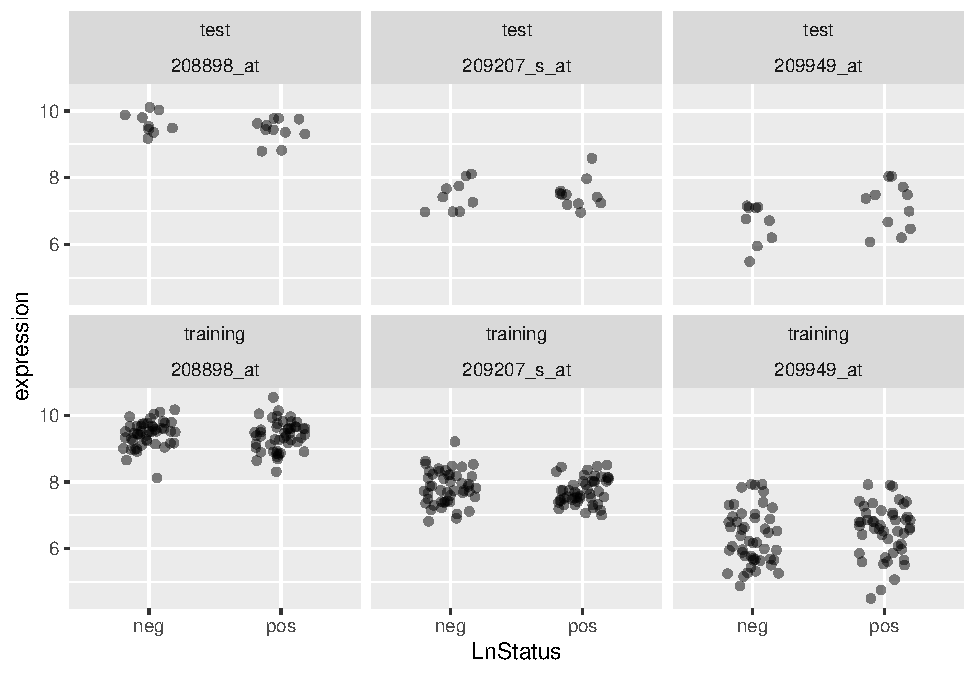
\includegraphics{Classification-of-disease-status-with-machine-learning-methods_files/figure-latex/scatterplot-1.pdf}

From the plot, it does not appear that one of these genes is
deferentially expressed across negative and positive \texttt{LnStatus}.
However, it is necessary to perform formal statistical test

\hypertarget{differential-expressionde-analysis}{%
\section{Differential expression(DE)
analysis}\label{differential-expressionde-analysis}}

The aim of DE analysis is to detect genes that are expressed with
significant differences across different conditions. One of the commonly
used approaches for this task is to employ linear regression, which
assesses one gene at a time to obtain its p-value. After that, the genes
that pass the significant threshold are selected. However, since the
number of genes can be in tens of thousands, it is essential to control
for the false positives. A common way to achieve this is by using the
Bonferroni correction to the p-value.

However, there is a problem with this approach - the gene expression
data is usually high dimensional, which means the number of measurements
is large compared to the sample size. Basically, this problem can lead
to an inflate in t-statistics and many false positives. The
\texttt{Limma} package specially solves this problem by adjusting the
t-statistics

\begin{Shaded}
\begin{Highlighting}[]
\NormalTok{designMatrix }\OtherTok{\textless{}{-}} \FunctionTok{model.matrix}\NormalTok{(}\SpecialCharTok{\textasciitilde{}}\NormalTok{LnStatus, }\AttributeTok{data =} \FunctionTok{pData}\NormalTok{(dat))}
\NormalTok{LMmodel }\OtherTok{\textless{}{-}}\NormalTok{ limma}\SpecialCharTok{::}\FunctionTok{lmFit}\NormalTok{(}\FunctionTok{exprs}\NormalTok{(dat), designMatrix)}
\NormalTok{LMmodelEb }\OtherTok{\textless{}{-}} \FunctionTok{eBayes}\NormalTok{(LMmodel)}
\end{Highlighting}
\end{Shaded}

The top \(10\) most statistically significant genes are the following:

\begin{Shaded}
\begin{Highlighting}[]
\FunctionTok{topTable}\NormalTok{(LMmodelEb)}
\end{Highlighting}
\end{Shaded}

\begin{verbatim}
## Removing intercept from test coefficients
\end{verbatim}

\begin{verbatim}
##                  logFC   AveExpr         t      P.Value adj.P.Val           B
## 208661_s_at -0.3847793 10.108683 -4.521262 1.468706e-05 0.3491816  1.43471257
## 205655_at   -0.6218631  5.261478 -4.247089 4.335858e-05 0.3491816  0.71985083
## 237746_at   -0.4480833  5.573586 -4.187085 5.463036e-05 0.3491816  0.56725204
## 229656_s_at  0.7837965  3.879888  4.155741 6.158687e-05 0.3491816  0.48810979
## 208663_s_at -0.4104289  9.257540 -4.114516 7.203779e-05 0.3491816  0.38462423
## 215307_at   -0.5994124  5.461940 -4.003212 1.094231e-04 0.3824809  0.10871177
## 228510_at   -0.3725724  4.974494 -4.000652 1.104706e-04 0.3824809  0.10242490
## 212384_at   -0.5195046  6.266492 -3.919799 1.489320e-04 0.4511896 -0.09464556
## 224872_at    0.2979676  8.331945  3.840721 1.986824e-04 0.5350297 -0.28466249
## 1556088_at  -0.3883365  4.984796 -3.791056 2.376244e-04 0.5679087 -0.40259597
\end{verbatim}

\hypertarget{fitting-the-classification-model}{%
\section{Fitting the Classification
model}\label{fitting-the-classification-model}}

In the study, the researchers utilized a support vector machine
classifier to differentiate between LN-positive and LN-negative tumors
through classification. They assessed the outcomes using ROC curves.
Following some optimization efforts, they achieved an area under the ROC
curve (AUC) of 0.66 on the training data set and 0.65 on the test set.
While these results surpass random chance, they do not provide strong
evidence regarding the significance of the derived molecular signature.
(Random chance would yield an AUC of 0.5, while perfect classification
would result in an AUC of 1.0).

In this section, we want to compare multiple classification models'
performance on this particular data set. We first employ
cross-validation to identify the optimal model for predicting in the
training set. We then select the best model to predict the
\texttt{LnStatus} in the test set and evaluate its performance.

\hypertarget{model-selection}{%
\subsection{Model selection}\label{model-selection}}

\begin{Shaded}
\begin{Highlighting}[]
\CommentTok{\#First Split the training set to perform cross{-}validation. By setting the argument strat = True, we ensure that each fold contains the same number of case and control samples. We also perform the cross{-}validation for 100 times by seting niter = 10.  }
\FunctionTok{set.seed}\NormalTok{(}\DecValTok{123}\NormalTok{)}
\NormalTok{splits }\OtherTok{\textless{}{-}}\NormalTok{ CMA}\SpecialCharTok{::}\FunctionTok{GenerateLearningsets}\NormalTok{(}\AttributeTok{y =}\NormalTok{ train.es}\SpecialCharTok{$}\NormalTok{LnStatus, }\AttributeTok{method=}\StringTok{"CV"}\NormalTok{, }\AttributeTok{fold=}\DecValTok{6}\NormalTok{, }\AttributeTok{strat=} \ConstantTok{TRUE}\NormalTok{, }\AttributeTok{niter =} \DecValTok{10}\NormalTok{)}
\end{Highlighting}
\end{Shaded}

Before testing the models, we first rank the genes by their significant
level in association with \texttt{Lnstatus}. We only use the top
features for the task of prediction. The function \texttt{Geneselection}
does this for each fold.

\begin{Shaded}
\begin{Highlighting}[]
\CommentTok{\#Rank the genes in term of p{-}value using the Limma method}
\NormalTok{Topgenes }\OtherTok{\textless{}{-}}\NormalTok{ CMA}\SpecialCharTok{::}\FunctionTok{GeneSelection}\NormalTok{(}\AttributeTok{X=}\FunctionTok{t}\NormalTok{(}\FunctionTok{exprs}\NormalTok{(train.es)), }\AttributeTok{y=}\NormalTok{train.es}\SpecialCharTok{$}\NormalTok{LnStatus, }\AttributeTok{learningsets=}\NormalTok{splits, }\AttributeTok{method=}\StringTok{"limma"}\NormalTok{)}
\end{Highlighting}
\end{Shaded}

In this example, I will compare the following classification methods:

\begin{itemize}
\item
  K-Nearest-Neighborhood(KNN).
\item
  Linear Discrimination Analysis(LDA).
\item
  Support Vector Machine(SVM)
\item
  Elastic net.
\item
  Random Forest.
\item
  Feed-Forward Neural Networks.
\item
  Probabilistic nearest neighbour.
\end{itemize}

\begin{Shaded}
\begin{Highlighting}[]
\FunctionTok{set.seed}\NormalTok{(}\DecValTok{123}\NormalTok{)}
\NormalTok{n }\OtherTok{\textless{}{-}} \DecValTok{50} \CommentTok{\#Number of top genes }
\CommentTok{\# Fitting the SVM model }
\NormalTok{pr\_SVM }\OtherTok{\textless{}{-}} \FunctionTok{classification}\NormalTok{(}\AttributeTok{X =} \FunctionTok{t}\NormalTok{(}\FunctionTok{exprs}\NormalTok{(train.es)), }\AttributeTok{y =}\NormalTok{ train.es}\SpecialCharTok{$}\NormalTok{LnStatus, }\AttributeTok{learningsets =}\NormalTok{ splits,}
\AttributeTok{genesel =}\NormalTok{ Topgenes, }\AttributeTok{nbgene =}\NormalTok{ n, }\AttributeTok{classifier =}\NormalTok{ svmCMA, }\AttributeTok{probability =} \ConstantTok{TRUE}\NormalTok{)}

\CommentTok{\#KNN}
\NormalTok{pr\_KNN }\OtherTok{\textless{}{-}} \FunctionTok{classification}\NormalTok{(}\AttributeTok{X =} \FunctionTok{t}\NormalTok{(}\FunctionTok{exprs}\NormalTok{(train.es)), }\AttributeTok{y =}\NormalTok{ train.es}\SpecialCharTok{$}\NormalTok{LnStatus, }\AttributeTok{learningsets =}\NormalTok{ splits,}
\AttributeTok{genesel =}\NormalTok{ Topgenes, }\AttributeTok{nbgene =}\NormalTok{ n, }\AttributeTok{classifier =}\NormalTok{ knnCMA)}

\CommentTok{\# LDA}
\NormalTok{pr\_LDA }\OtherTok{\textless{}{-}} \FunctionTok{classification}\NormalTok{(}\AttributeTok{X =} \FunctionTok{t}\NormalTok{(}\FunctionTok{exprs}\NormalTok{(train.es)), }\AttributeTok{y =}\NormalTok{ train.es}\SpecialCharTok{$}\NormalTok{LnStatus, }\AttributeTok{learningsets =}\NormalTok{ splits,}
\AttributeTok{genesel =}\NormalTok{ Topgenes, }\AttributeTok{nbgene =}\NormalTok{ n, }\AttributeTok{classifier =}\NormalTok{ ldaCMA)}

\CommentTok{\# Elastic Net}
\NormalTok{pr\_EN }\OtherTok{\textless{}{-}} \FunctionTok{classification}\NormalTok{(}\AttributeTok{X =} \FunctionTok{t}\NormalTok{(}\FunctionTok{exprs}\NormalTok{(train.es)), }\AttributeTok{y =}\NormalTok{ train.es}\SpecialCharTok{$}\NormalTok{LnStatus, }\AttributeTok{learningsets =}\NormalTok{ splits,}
\AttributeTok{genesel =}\NormalTok{ Topgenes, }\AttributeTok{nbgene =}\NormalTok{ n, }\AttributeTok{classifier =}\NormalTok{ ElasticNetCMA)}

\CommentTok{\#Random forest}
\NormalTok{pr\_RF }\OtherTok{\textless{}{-}} \FunctionTok{classification}\NormalTok{(}\AttributeTok{X =} \FunctionTok{t}\NormalTok{(}\FunctionTok{exprs}\NormalTok{(train.es)), }\AttributeTok{y =}\NormalTok{ train.es}\SpecialCharTok{$}\NormalTok{LnStatus, }\AttributeTok{learningsets =}\NormalTok{ splits,}
\AttributeTok{genesel =}\NormalTok{ Topgenes, }\AttributeTok{nbgene =}\NormalTok{ n, }\AttributeTok{classifier =}\NormalTok{ rfCMA)}
\end{Highlighting}
\end{Shaded}

\begin{verbatim}
## Warning: package 'randomForest' was built under R version 4.3.3
\end{verbatim}

\begin{Shaded}
\begin{Highlighting}[]
\CommentTok{\#Feed{-}Forward Neural Networks}
\NormalTok{pr\_FNN }\OtherTok{\textless{}{-}} \FunctionTok{classification}\NormalTok{(}\AttributeTok{X =} \FunctionTok{t}\NormalTok{(}\FunctionTok{exprs}\NormalTok{(train.es)), }\AttributeTok{y =}\NormalTok{ train.es}\SpecialCharTok{$}\NormalTok{LnStatus, }\AttributeTok{learningsets =}\NormalTok{ splits,}
\AttributeTok{genesel =}\NormalTok{ Topgenes, }\AttributeTok{nbgene =}\NormalTok{ n, }\AttributeTok{classifier =}\NormalTok{ nnetCMA)}

\CommentTok{\#Probabilistic nearest neighbours}
\NormalTok{pr\_PNN }\OtherTok{\textless{}{-}} \FunctionTok{classification}\NormalTok{(}\AttributeTok{X =} \FunctionTok{t}\NormalTok{(}\FunctionTok{exprs}\NormalTok{(train.es)), }\AttributeTok{y =}\NormalTok{ train.es}\SpecialCharTok{$}\NormalTok{LnStatus, }\AttributeTok{learningsets =}\NormalTok{ splits,}
\AttributeTok{genesel =}\NormalTok{ Topgenes, }\AttributeTok{nbgene =}\NormalTok{ n, }\AttributeTok{classifier =}\NormalTok{ pknnCMA)}
\end{Highlighting}
\end{Shaded}

Let us make a comparison using multiple metrics:

\begin{itemize}
\item
  Misclassification: The proportion of data that are labelled
  incorrectly.
\item
  Sensitivity: the proportion of actual positives which are correctly
  identified.
\item
  Specificity: the proportion of actual negatives which are correctly
  identified.
\item
  AUC: The area under the ROC(Receiver Operating Characteristic) curve.
  A ROC curve plots the true positive rate (sensitivity) against the
  false positive rate (1 - specificity) at different decision
  thresholds. An AUC value closer to 1 indicates a better model
  performance.
\end{itemize}

In medical contexts, there are situations where it is crucial to
prioritize either high sensitivity or high specificity when selecting a
model. For instance, in cancer diagnostics, achieving high sensitivity
is paramount because misdiagnosing individuals with cancer can miss the
opportunity for timely treatment.

Let us now compare the model's performance using these metrics.

\begin{Shaded}
\begin{Highlighting}[]
\NormalTok{pr }\OtherTok{\textless{}{-}} \FunctionTok{list}\NormalTok{(pr\_SVM, pr\_KNN, pr\_LDA, pr\_EN, pr\_RF, pr\_FNN, pr\_PNN)}
\NormalTok{comparison }\OtherTok{\textless{}{-}} \FunctionTok{compare}\NormalTok{(pr, }\AttributeTok{plot =} \ConstantTok{TRUE}\NormalTok{, }\AttributeTok{measure =} \FunctionTok{c}\NormalTok{(}\StringTok{"misclassification"}\NormalTok{, }\StringTok{"sensitivity"}\NormalTok{, }\StringTok{"specificity"}\NormalTok{))}
\end{Highlighting}
\end{Shaded}

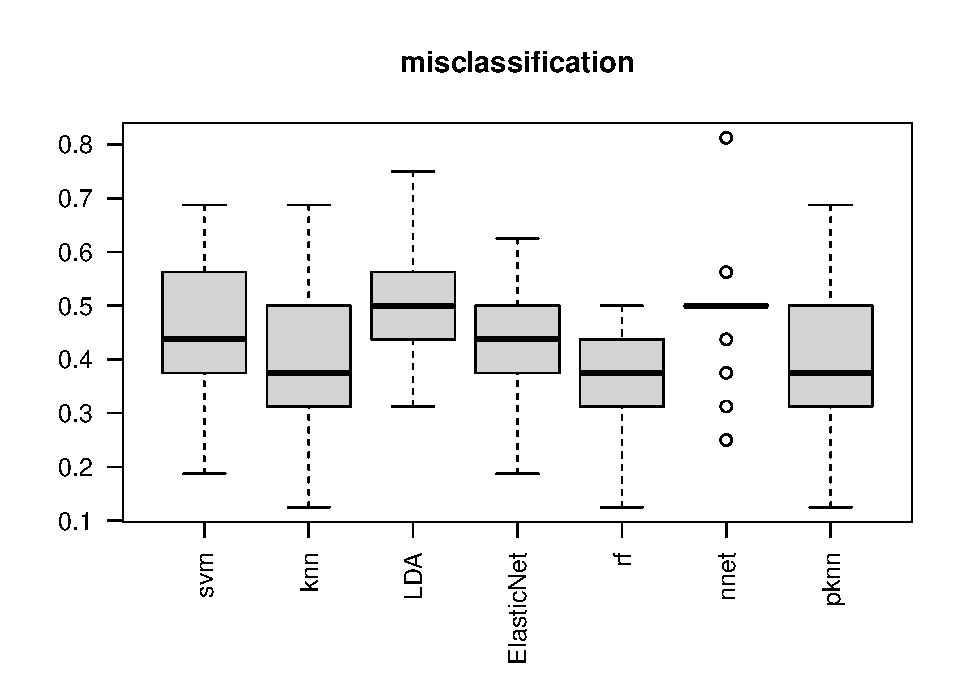
\includegraphics{Classification-of-disease-status-with-machine-learning-methods_files/figure-latex/compare-1.pdf}
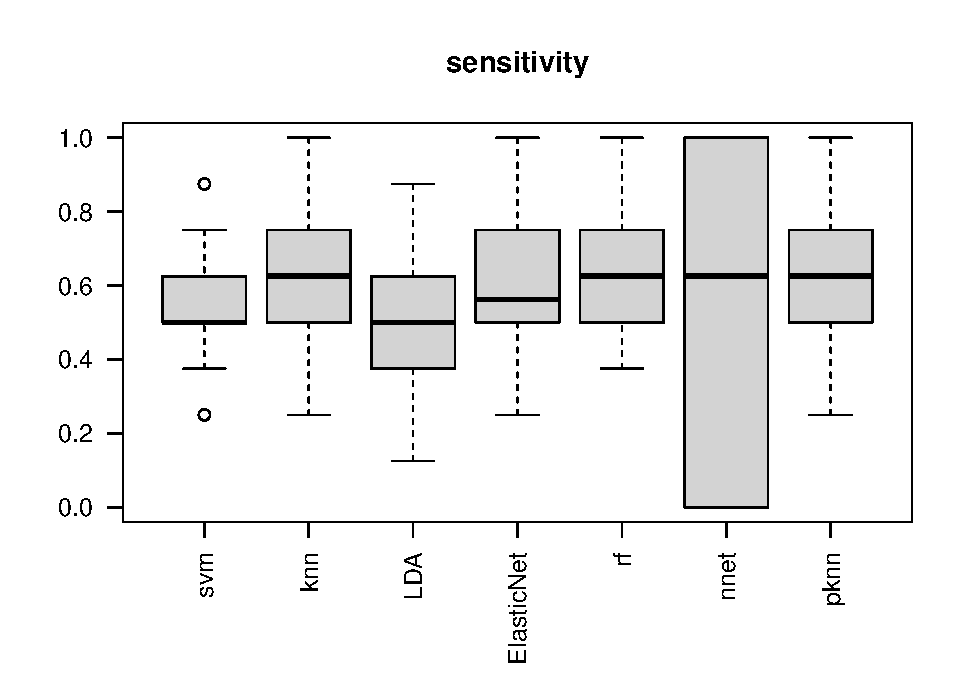
\includegraphics{Classification-of-disease-status-with-machine-learning-methods_files/figure-latex/compare-2.pdf}
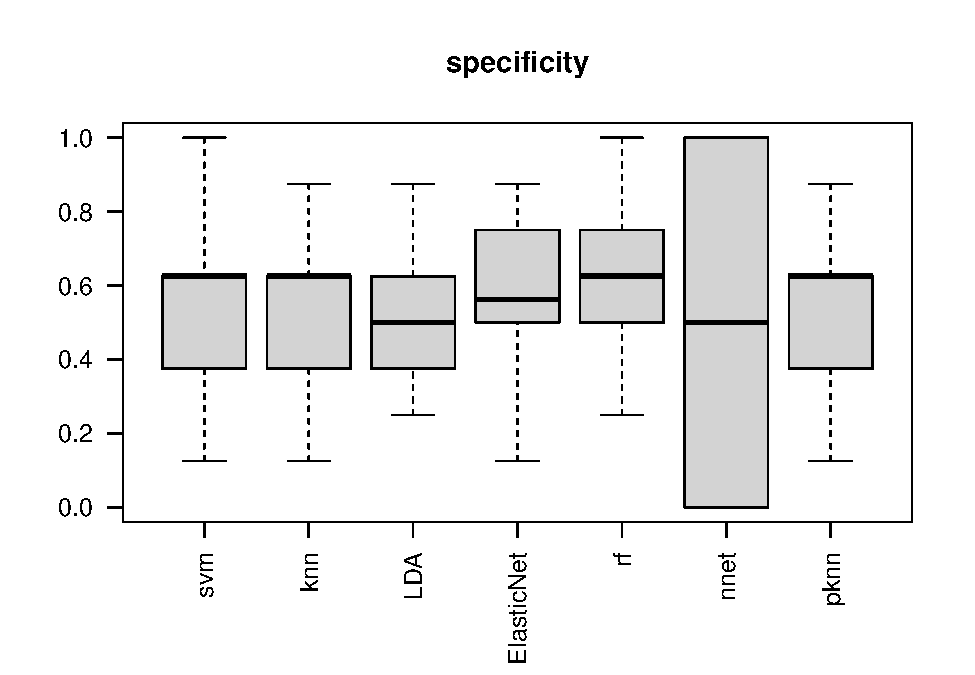
\includegraphics{Classification-of-disease-status-with-machine-learning-methods_files/figure-latex/compare-3.pdf}

\begin{Shaded}
\begin{Highlighting}[]
\FunctionTok{print}\NormalTok{(comparison)}
\end{Highlighting}
\end{Shaded}

\begin{verbatim}
##            misclassification sensitivity specificity
## svm                0.4364583   0.5604167   0.5666667
## knn                0.4125000   0.6250000   0.5500000
## LDA                0.4947917   0.5083333   0.5020833
## ElasticNet         0.4187500   0.5812500   0.5812500
## rf                 0.3677083   0.6562500   0.6083333
## nnet               0.4895833   0.5312500   0.4895833
## pknn               0.4125000   0.6250000   0.5500000
\end{verbatim}

We see that random forest achieves the lowest mis-classification rate.
It also has the highest sensitivity and specificity among all models as
well.

\begin{Shaded}
\begin{Highlighting}[]
\CommentTok{\#Compare the auc metric}
\NormalTok{pr2 }\OtherTok{\textless{}{-}} \FunctionTok{list}\NormalTok{(pr\_LDA, pr\_EN, pr\_RF, pr\_FNN, pr\_PNN, pr\_SVM)}
\NormalTok{comparison2 }\OtherTok{\textless{}{-}} \FunctionTok{compare}\NormalTok{(pr2, }\AttributeTok{measure =} \FunctionTok{c}\NormalTok{(}\StringTok{"auc"}\NormalTok{))}
\FunctionTok{print}\NormalTok{(comparison2)}
\end{Highlighting}
\end{Shaded}

\begin{verbatim}
##                  auc
## LDA        0.5239583
## ElasticNet 0.5986979
## rf         0.6544271
## nnet       0.5020833
## pknn       0.4455729
## svm        0.5812500
\end{verbatim}

It looks like that random forest method has the highest AUC. Based on
all metrics, we conclude that random forest is the best classification
model for this data set. Note this AUC is the same as what the authors
achieved in their training set. Let us now evaluate it on the test set
and see if there is any improvement.

\hypertarget{testing-the-selected-model}{%
\subsection{Testing the selected
model}\label{testing-the-selected-model}}

Now that we decided on which method we are going to use to classify
samples in the test set, we need to train the model using the full
training set and then classify samples of the test set.

\begin{Shaded}
\begin{Highlighting}[]
\CommentTok{\#Selecting the top 50 significant genes selected by the package Limma}
\NormalTok{inx }\OtherTok{\textless{}{-}} \FunctionTok{rownames}\NormalTok{(}\FunctionTok{topTable}\NormalTok{(LMmodelEb, }\AttributeTok{number =} \DecValTok{50}\NormalTok{))}
\NormalTok{train\_exprsmat }\OtherTok{\textless{}{-}} \FunctionTok{exprs}\NormalTok{(train.es)[inx,]}
\NormalTok{test\_exprsmat }\OtherTok{\textless{}{-}} \FunctionTok{exprs}\NormalTok{(test.es)[inx,]}
\end{Highlighting}
\end{Shaded}

\begin{Shaded}
\begin{Highlighting}[]
\CommentTok{\#Fitting the model}
\FunctionTok{set.seed}\NormalTok{(}\DecValTok{344}\NormalTok{)}
\NormalTok{RF }\OtherTok{\textless{}{-}} \FunctionTok{randomForest}\NormalTok{(}\AttributeTok{x =} \FunctionTok{t}\NormalTok{(train\_exprsmat), }\AttributeTok{y =}\NormalTok{ train.es}\SpecialCharTok{$}\NormalTok{LnStatus, }\AttributeTok{xtest =} \FunctionTok{t}\NormalTok{(test\_exprsmat), }\AttributeTok{ytest =}\NormalTok{ test.es}\SpecialCharTok{$}\NormalTok{LnStatus)}

\CommentTok{\#Store the prediction value}
\NormalTok{yhat.RF }\OtherTok{\textless{}{-}}\NormalTok{ RF}\SpecialCharTok{$}\NormalTok{test}\SpecialCharTok{$}\NormalTok{predicted}

\CommentTok{\#Calculate the misclassification rate}
\NormalTok{pr.errTest}\OtherTok{\textless{}{-}} \FunctionTok{mean}\NormalTok{(test.es}\SpecialCharTok{$}\NormalTok{LnStatus }\SpecialCharTok{!=}\NormalTok{ yhat.RF)}
\NormalTok{pr.errTest}
\end{Highlighting}
\end{Shaded}

\begin{verbatim}
## [1] 0.35
\end{verbatim}

This is comparable to the misclassification rate obtained by the
cross-validation(0.368).

\begin{Shaded}
\begin{Highlighting}[]
\CommentTok{\#Calculate the sensitivity and Specificity}
\NormalTok{sensitivity }\OtherTok{\textless{}{-}} \FunctionTok{sum}\NormalTok{(yhat.RF[test.es}\SpecialCharTok{$}\NormalTok{LnStatus }\SpecialCharTok{==} \StringTok{"pos"}\NormalTok{] }\SpecialCharTok{==} \StringTok{"pos"}\NormalTok{)}\SpecialCharTok{/} \FunctionTok{sum}\NormalTok{(test.es}\SpecialCharTok{$}\NormalTok{LnStatus }\SpecialCharTok{==} \StringTok{"pos"}\NormalTok{) }
\NormalTok{specificity }\OtherTok{\textless{}{-}} \FunctionTok{sum}\NormalTok{(yhat.RF[test.es}\SpecialCharTok{$}\NormalTok{LnStatus }\SpecialCharTok{==} \StringTok{"neg"}\NormalTok{] }\SpecialCharTok{==} \StringTok{"neg"}\NormalTok{)}\SpecialCharTok{/} \FunctionTok{sum}\NormalTok{(test.es}\SpecialCharTok{$}\NormalTok{LnStatus }\SpecialCharTok{==} \StringTok{"neg"}\NormalTok{)}
\FunctionTok{print}\NormalTok{(sensitivity); }\FunctionTok{print}\NormalTok{(specificity)}
\end{Highlighting}
\end{Shaded}

\begin{verbatim}
## [1] 0.7272727
\end{verbatim}

\begin{verbatim}
## [1] 0.5555556
\end{verbatim}

\begin{Shaded}
\begin{Highlighting}[]
\CommentTok{\#Plot the ROC curve and compute the AUC}
\NormalTok{roc\_obj }\OtherTok{\textless{}{-}} \FunctionTok{roc}\NormalTok{(test.es}\SpecialCharTok{$}\NormalTok{LnStatus,  RF}\SpecialCharTok{$}\NormalTok{test}\SpecialCharTok{$}\NormalTok{votes[,}\DecValTok{2}\NormalTok{] )}
\FunctionTok{plot}\NormalTok{(roc\_obj,}\AttributeTok{main =} \StringTok{"ROC curve of random forest classification"}\NormalTok{)}
\end{Highlighting}
\end{Shaded}

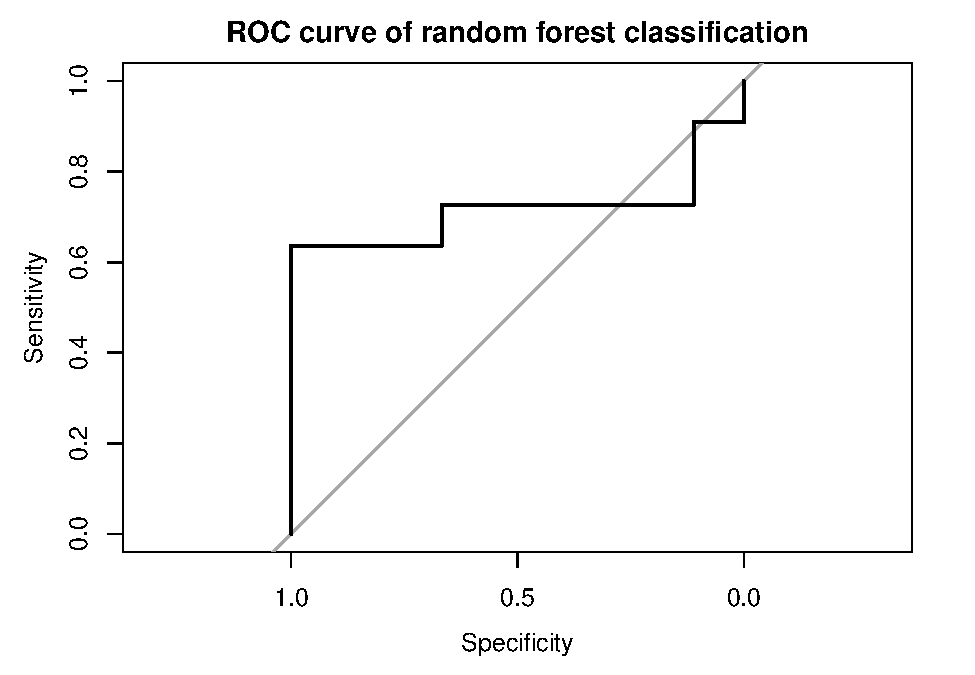
\includegraphics{Classification-of-disease-status-with-machine-learning-methods_files/figure-latex/unnamed-chunk-12-1.pdf}

\begin{Shaded}
\begin{Highlighting}[]
\FunctionTok{auc}\NormalTok{(roc\_obj)}
\end{Highlighting}
\end{Shaded}

\begin{verbatim}
## Area under the curve: 0.7172
\end{verbatim}

The ROC plot illustrates that most data points are positioned above the
diagonal line, which indicates a higher proportion of true positives
compared to false positives. The Area Under the Curve (AUC) metric
quantifies the overall performance of the model by calculating the area
under the ROC curve. The AUC value is calculated to be 0.717, which is
higher than what was achieved during cross-validation and what the
authors achieved in their publication.

\hypertarget{conclusion}{%
\section{Conclusion}\label{conclusion}}

We initiated our analysis by conducting inference on the data set to
identify genes significantly associated with disease status.
Subsequently, we utilized these genes to predict the disease status of
test samples by leveraging the top 50 gene expressions. Our study
involved the comparison of various machine learning methods through
cross-validation, revealing that the random forest algorithm exhibited
superior performance across all metrics (mis-classification rate of
0.368, sensitivity of 0.656, specificity of 0.608).

Further evaluation of the random forest model on the test set yielded an
AUC value of 0.717, demonstrating a slight enhancement in performance
compared to existing literature. However, in the context of cancer
diagnostics, sensitivity emerges as a critical metric. With a
sensitivity of 0.656, our model wrongly diagnoses an average of 34 out
of 100 true cancer patients. This is not good enough to be of clinical
relevance.

Considering the prevalence of lymph-node-positive breast cancer, which
is approximately 33\% during diagnosis (according to
{[}\url{http://seer.cancer.gov/statfacts/html/breast.html}{]}), it is
crucial to build a model with high sensitivity (close to 1). Given that
both our best model and the authors' model achieve similar performance,
it is likely that additional data, such as patient information, is
essential to enhance prediction accuracy and clinical utility.

\end{document}
